\subsection{Ca sử dụng tổng hợp lịch trình từ hội thoại}
\vspace{0.5cm}


\noindent 
\begin{tabularx}{\linewidth}{| l | X |} 
\hline 
\textbf{Mô tả} & Hệ thống sẽ tổng hợp lại lịch trình được đúc kết từ đoạn tin nhắn trong nhóm chat của người dùng.  \\ 
\hline 
\textbf{Luồng cơ bản} & 1. Người dùng bấm vào một cuộc hội thoại nhóm muốn tổng hợp. \newline
                        2. Hệ thống hiển thị thông cuộc hội thoại và các tin nhắn trong cuộc hội thoại đó. \newline
                        3. Người dùng chọn tùy chọn tổng hợp tin nhắn. \newline
                        4. Hệ thống lấy và hiển thị lịch trình tổng hợp của cuộc hội thoại (nếu có) . \newline
                        5. Người dùng bấm "Tổng hợp". \newline
                        6. Hệ thống sử dụng AI tổng hợp lịch trình trong cuộc hội thoại và hiển thị lịch trình tổng hợp. \\
                        
\hline 
\textbf{Luồng thay thế} & Hệ thống thông báo lỗi khi không có tin nhắn mới chưa được cập nhật. \\

                       
\hline 
\textbf{Tiền điều kiện} &- Người dùng đang đăng nhập và phiên đăng nhập chưa kết thúc. \newline
                        - Người dùng đã có ít nhất một cuộc hội thoại nhóm. \\
\hline 
\textbf{Hậu điều kiện} & - Hệ thống tổng hợp lịch trình sau đó lưu vào cơ sở dữ liệu và hiển thị cho người dùng. \newline
                        - Hệ thống đánh dấu các tin nhắn đã được tổng hợp. \newline
                        - Hệ thống gộp lịch trình với lịch trình đã tổng hợp trước đó.\\

\hline 
\textbf{Yêu cầu phi chức năng} & Hệ thống xử lý tổng hợp lịch trình dưới 10s  \\ 
\hline 
\end{tabularx}



\noindent 
\begin{tabular}{| c | c |}
    \hline
    \textbf{Biểu đồ hoạt động} & \textbf{Quan hệ} \\ 
    \hline
    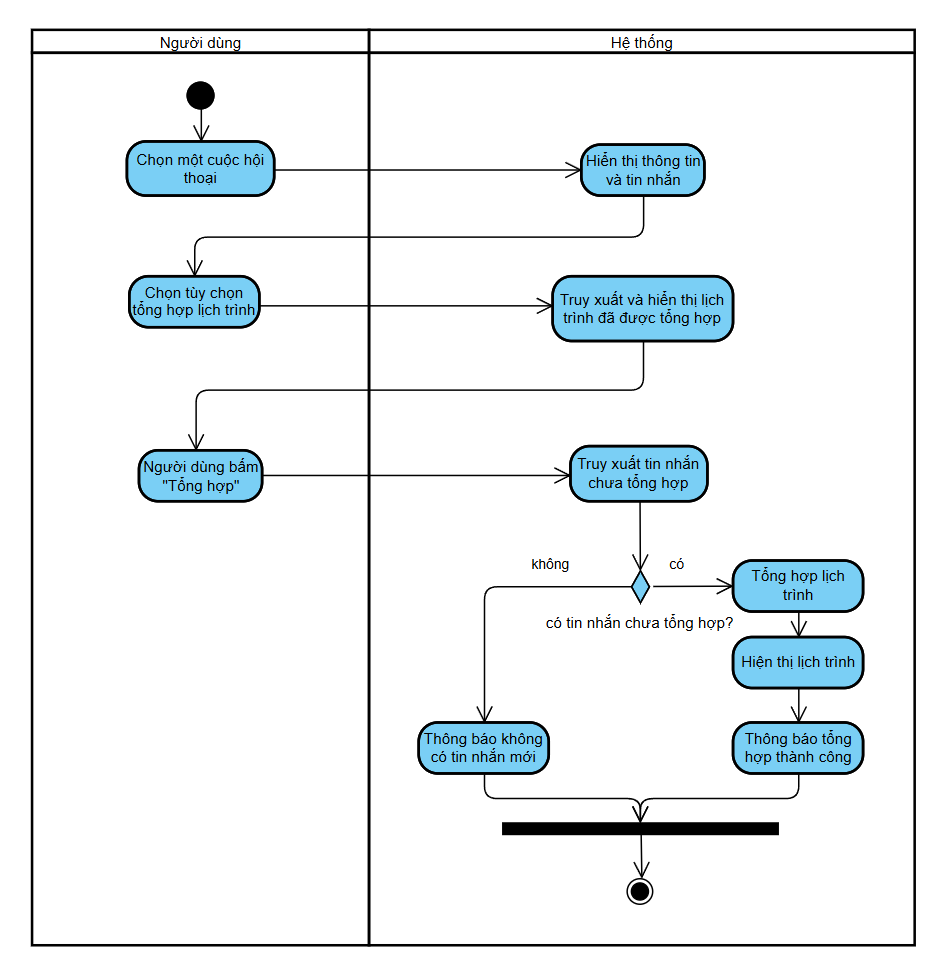
\includegraphics[width=0.5\linewidth]{figures/c3/3-3-10-ad.png} 
    & 
    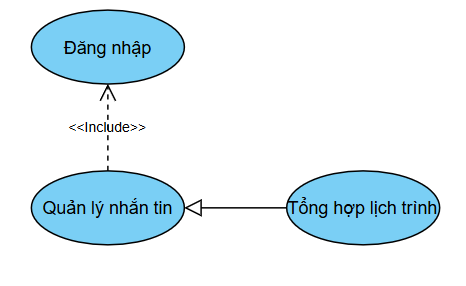
\includegraphics[width=0.45\linewidth]{figures/c3/3-3-10-rd.png} \\ 
    \hline
\end{tabular}


\vspace{0.8cm}

\begin{figure}[H]
    \centering  
    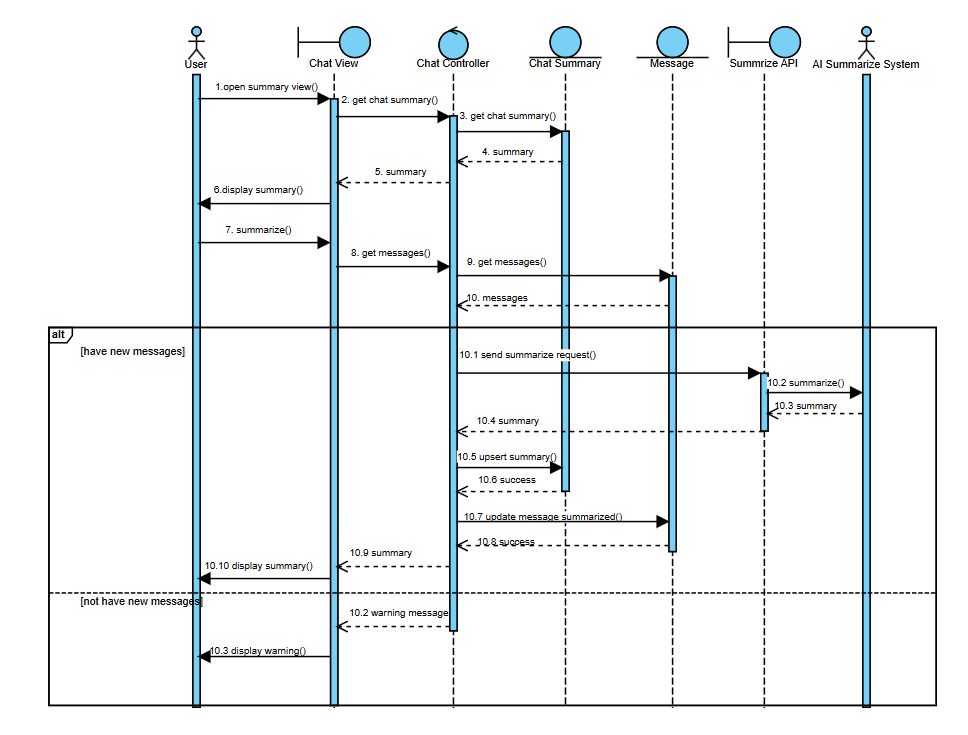
\includegraphics[width=1\textwidth]{figures/c3/3-3-10-sd.png}
    \caption{Biểu đồ tuần tự ca sử dụng tổng hợp lịch trình.}
    \label{fig:3-3-10-sequence-diagram}
\end{figure}